\documentclass[a4paper]{article}

\usepackage[francais]{babel}
\usepackage{amsmath}
\usepackage{amssymb}
\usepackage{graphicx}
%\usepackage{algorithmic}
\usepackage{url}
%\usepackage{subfig}
%\usepackage[squaren,Gray]{SIunits}

% reduce margin.
\usepackage[]{fullpage}

\makeatletter
\def\thickhrulefill{\leavevmode \leaders \hrule height 1pt\hfill \kern \z@}
\def\maketitle{
  \null
  \thispagestyle{empty}
  \vskip 1cm
  \begin{flushright}
	\normalfont\Large\@author
  \end{flushright}
  \vfil
  \hrule height 2pt
  \par
  \begin{center}
	\huge \strut \@title \par
  \end{center}
  \hrule height 2pt
  \par
  \vfil
  \vfil
  \null
\begin{center}
\end{center}
\begin{figure}[!ht]
	\centering
	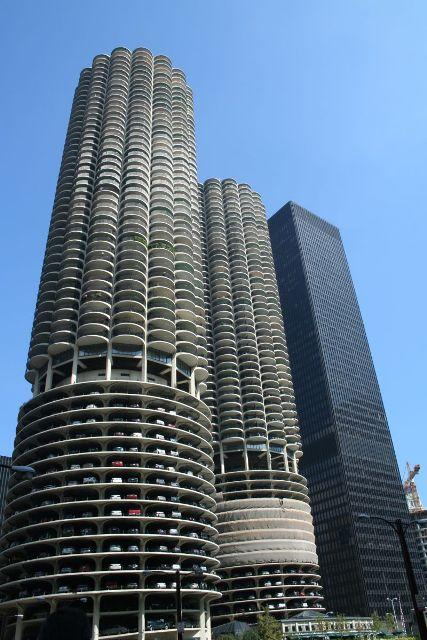
\includegraphics[scale=.5]{imgs/parkingpres.jpg}
\end{figure}
\begin{figure}[!ht]
	\centering
	
\includegraphics[scale=.5]{imgs/polytech.png}
\end{figure}
\vfil
  \cleardoublepage
  }
\makeatother
\author{Fran\c cois Chapuis, Roman Mkrtchian, K\'evin Rocher, Mathieu Bivert}
\title{Conception Objet: Mod\'elisation d'un parking \`a p\'eage}
\date{Ann\'ee scolaire $2011$-$2012$}

\begin{document}
\maketitle
\newpage
\tableofcontents
\newpage

\section{Pr\'esentation}
Ce document a pour but de r\'ealiser une mod\'elisation objet d'un parking \`a p\'eage.
Pour ce faire, on commencera par d\'ecrire de fa\c con g\'en\'erale le fonctionnement
du syst\`eme, pour ensuite rentrer dans les d\'etails via diff\'erents types de diagrammes
\'etudi\'es en cours\footnote{\url{http://users.polytech.unice.fr/~cm/}}.

\section{Description du syst\`eme}
Le parking, repr\'esent\'e figure \ref{parking}, est compos\'e de plusieurs entr\'ees,
sorties et caisses.
\begin{figure}[!ht]
	\centering
	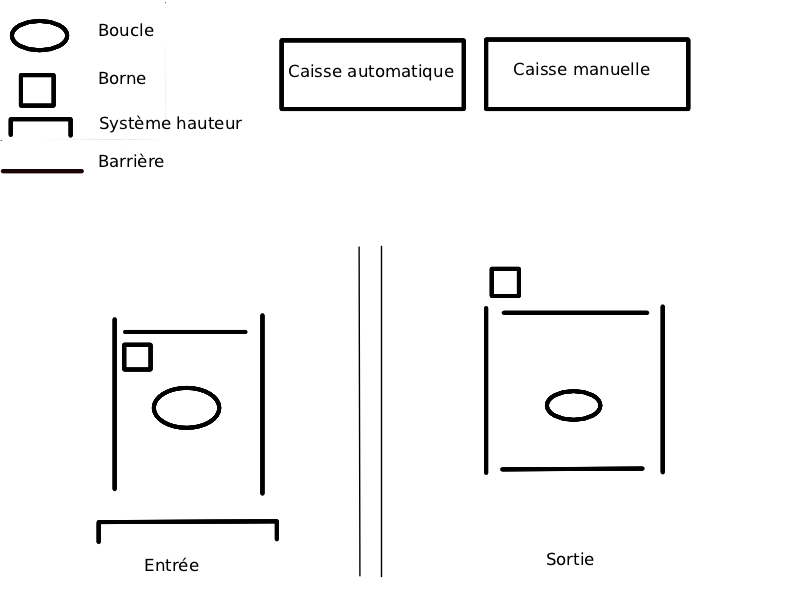
\includegraphics[scale=.6]{imgs/parking.png}
	\caption{\label{parking} Sch\'ema du parking. Pour simplifier, les \'el\'ements
		dupliqu\'es ne sont repr\'esent\'es qu'une seule fois}
\end{figure}
Les bornes sont elles-m\^emes compos\'ees de plusieurs \'el\'ements.
\begin{figure}[!ht]
	\centering
	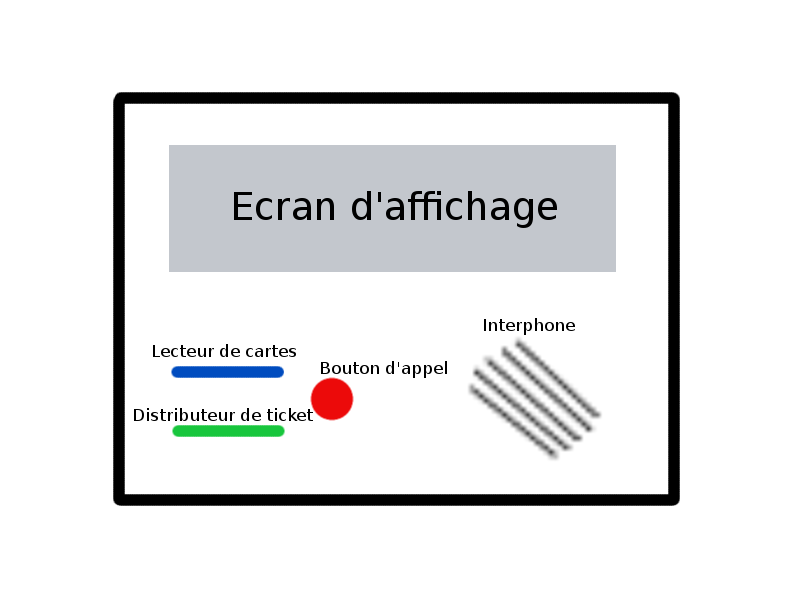
\includegraphics[scale=.4]{imgs/borne.png}
	\caption{\label{borne} Sch\'ema d'une borne, contenant un lecteur de carte,
	un distributeur de tickets, un interphone ainsi qu'un bouton d'appel.}
\end{figure}

Une entr\'ee est typiquement constitu\'ee de :
\begin{description}
	\item[une boucle] au sol, permettant d'obtenir le poids magn\'etique du v\'ehicule
		passant dessus;
	\item[une barri\`ere] r\'egulant l'entr\'ee du parking;
	\item[une borne] compos\'ee d'un interphone, d'un distributeur de ticket et d'un
		lecteur de cartes;
	\item[un syst\`eme de limitation en hauteur], afin de refuser l'entr\'ee aux
		v\'ehicules trop imposants.
\end{description}

La borne situ\'ee \`a l'entr\'ee permet soit d'obtenir un ticket magn\'etique, soit de
prendre l'empreinte d'une carte bancaire ou encore d'une carte d'abonnement. Ce sont,
comme on le verra plus tard, les trois grands moyens de payements mis en \o euvre. De
plus, la pr\'esence d'un interphone permet de contacter un employ\'e du parking en
cas de besoin.

Une sortie a une composition similaire \`a celle d'une entr\'ee, au d\'etail pr\`es
qu'elle dispose de deux barri\`eres, et que le syst\`eme de limitation en hauteur
lui a \'et\'e retir\'e.

On distingue deux types de caisses: les caisses automatiques ainsi qu'une caisse
manuelle.

\subsection{Acteurs}
On identifie plusieurs acteurs pouvant int\'eragir au niveau du parking:
\begin{itemize}
	\item Le client;
	\item le surveillant du parking;
	\item le technicien;
	\item la banque;
	\item la fourri\`ere;
	\item la soci\'et\'e g\'erant le parking.
\end{itemize}

\subsubsection{Client}
Les clients sont class\'es en trois cat\'egories, selon la fa\c con qu'ils ont choisie
pour rentrer dans le parking, \`a savoir:
\begin{itemize}
	\item les clients abonn\'es, utilisant une carte d'abonnement;
	\item les clients rentrant \`a l'aide d'une carte bancaire;
	\item les autres clients, c'est \`a dire ceux qui ont r\'ecup\'er\'e un
		ticket magn\'etique.
\end{itemize}
\subsubsection{Surveillant du parking}
Il est charg\'e de v\'erifier et d'approvisionner les bornes ainsi que les caisses
de payements en consommables (papier, monnaie, $\hdots$). C'est \`a lui que les
clients vont parler lorsqu'ils d\'ecident d'utiliser un des interphones situ\'es sur
les bornes. De plus, c'est l'acteur charg\'e de communiquer au technicien les \'eventuelles
d\'efaillances techniques, ou encore de pr\'evenir la fourri\`ere en cas de stationnement
prolong\'e d'un v\'ehicule.

Enfin, le surveillant est charg\'e de s'occuper de la caisse manuelle.

\subsubsection{Technicien}
C'est \`a lui qu'incombe la t\^ache de v\'erifier et d'entretenir les diff\'erents
composants du parking (barri\`ere, borne, $\hdots$). Il est pr\'evenu par le surveillant
en cas de probl\`eme. 

Selon la taille du parking et les besoins de la soci\'et\'e de parking, les r\^oles
de surveillant et de technicien peuvent bien entendu \^etre occup\'es par la m\^eme
personne.

\subsubsection{Banque}
\`A la fin de la journ\'ee, toutes les transactions bancaires lui sont envoy\'ees. Elle
a pour r\^ole de les r\'ecuperer et de le traiter.

\subsubsection{Fourri\`ere}
Si un v\'ehicule est stationn\'e sur le parking depuis au moins $72$ heures dans l'enceinte
du parking, la fourri\`ere a de fortes chances d'\^etre appell\'ee par le surveillant afin
de venir r\'ecuperer le v\'ehicule.

\subsubsection{Soci\'et\'e de parking}
C'est elle qui poss\`ede et g\`ere le parking. Elle intervient ici essentiellement pour
recevoir les statistiques sur l'utilisation du parking, envoy\'e une fois par jour, au
m\^eme moment que les transactions bancaires.

\subsection{Fonctionnalit\'es}
Les acteurs vont int\'eragir sur le syst\`eme au travers de deux grandes fonctionnalit\'es:
\begin{enumerate}
	\item \textit{Se garer};
	\item \textit{Gestion du parking}.
\end{enumerate}


Les sc\'enarios Cokburn donnent une description plus pr\'ecise et compl\`ete des diff\'erents
\'elements de ces fonctionnalit\'es.

\section{Diagrammes des cas d'utilisation (Use case) et sc\'enarios brefs}
La figure \ref{usecase} repr\'esente le diagramme des cas d'utilisation
de haut niveau. Il contient les deux fonctionalit\'es identifi\'ees plus
haut (se garer et la gestion du parking) ainsi que les utilisateurs
d\'efinis auparavant.
\begin{figure}[!ht]
	\centering
	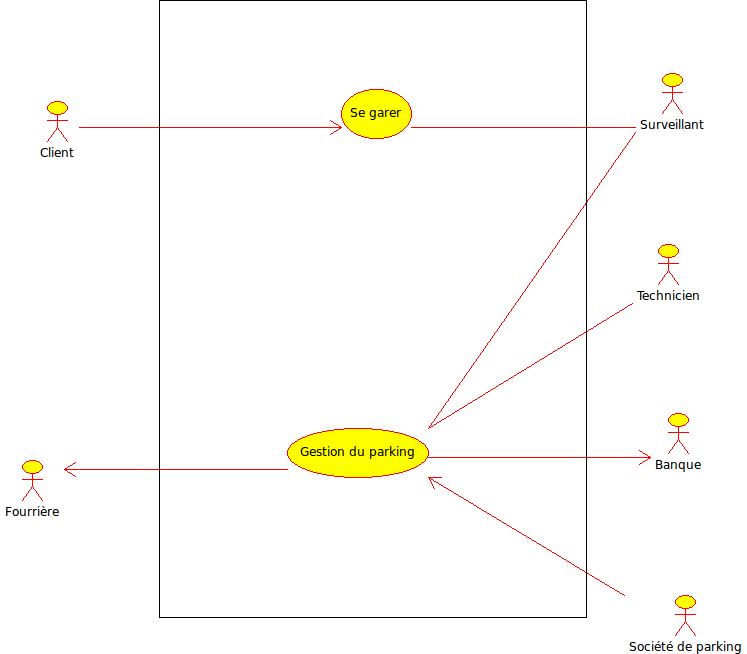
\includegraphics[scale=.7]{parking.png}
	\caption{\label{usecase} Diagramme des cas d'utilisation de haut niveau}
\end{figure}
\newpage
\subsection{Sc\'enarios brefs}
\subsubsection{Se garer}
Le client doit d'abord entrer dans le parking, pour cela il doit s'identifier pour pouvoir ensuite payer, il peut alors :
\begin{itemize}
		\item Prendre un ticket magn\'etique d'entr\'ee qui contiendra les informations sur l'heure d'entr\'ee et permettra ensuite de payer \`a une borne de paiment;
		\item Ins\'erer une carte d'abonnement d\'ej\`a cr\'edit\'ee qui sera d\'ebit\'ee automatiquement lorsque le client devra sortir;
		\item Ins\'erer une carte bancaire dont la signature magn\'etique sera identifi\'ee et qui pourra ensuite \^etre d\'ebit\'ee lors de la sortie.
\end{itemize}

Ensuite, une fois que le client veut partir, il doit payer. Pour cela il peut :
\begin{itemize}
		\item Ins\'erer la carte d'abonnement pour sortir, celle-ci sera d\'ebit\'ee automatiquement;
		\item Ins\'erer la m\^eme carte bancaire qu'il avait ins\'er\'e en entrant, et celle-ci sera \'egalement d\'ebit\'ee du montant ad\'equat;
		\item Ins\'erer le ticket d'entr\'ee dans une borne de paiment, payer avec un moyen de paiment tiers, et prendre le ticket magn\'etique de sortie qui permettra la lev\'ee de la barri\`ere;
\end{itemize}

\subsubsection{Gestion du parking}
Le parking a besoin d'etre maintenu et g\'er\'e. On distingue plusieurs aspects :
\begin{itemize}
		\item La gestion g\'en\'erale du parking et la coh\'erence de son fonctionnement assur\'ee par un surveillant;
		\item Le fait d'alimenter en consommable les machines et en monnaie les bornes de paiment.
		\item L'intervention d'un technicien en cas de panne des machines;
		\item L'envoi quotidien \`a la soci\'et\'e des informations relatives aux clients dans le but d'\'etablir des statistiques et les diff\'erentes transactions bancaires \`a effectuer;
\end{itemize}

% a réintégrer
% \section{Gestion du parking}
% \subsection{Cockburn}
% \begin{description}
% 	\item[Cas d'utilisation] gestion du parking
% 	\item[Acteur primaire] le syst\`eme
% 	\item[Acteur support]  la fourri\`ere, le surveillant, le technicien, soci\'et\'e
% 				de parking
% 	\item[Pr\'econdition] 
% 	\item[Sc\'enario Primaire] \
% 	\begin{enumerate}
% 		\item Le surveillant appelle la fourri\`ere si un v\'ehicule est
% 			pr\'esent sur le parking depuis plus de $72$ heures;
% 		\item le surveillant appelle le technicien en cas de probl\`emes
% 			techniques sur le parking;
% 		\item le technicien maintient r\'eguli\`erement les diff\'erents
% 			\'el\'ements du parking;
% 		\item le surveillant s'occupe d'alimenter les machines en consommables
% 			lorsque celles-ci lui signalent un manque;
% 		\item le surveillant alimente r\'eguli\`erement les caisses en
% 			monnaie et les bornes en consommables;
% 		\item le syst\`eme envoie quotidiennement \`a la soci\'et\'e des
% 			informations relatives aux clients (dans le but d'\'etablir des
% 			statistiques);
% 		\item le syst\`eme envoie quotidiennement \`a la soci\'et\'e les
% 			diff\'erentes transactions bancaires \`a effectuer.
% 	\end{enumerate}
% 	\item[Postcondition] les probl\`emes, s'il y en a, sont r\'esolus
% 	\item[Variantes] \
% \end{description}

\section{Le client se gare}
\subsection{Cockburn}
\begin{description}
	\item[Cas d'utilisation] le client se gare
	\item[Acteur primaire] client
	\item[Acteur support] surveillant
	\item[Pr\'econdition] place libre dans le parking
	\item[Sc\'enario Primaire] \
	\begin{enumerate}
		\item \textbf{le client rentre};
		\item \textbf{le client paye};
		\item \textbf{le client sort}.
	\end{enumerate}
	\item[Postcondition] le client s'est gar\'e, a pay\'e et est sorti du parking
\end{description}

\subsection{Diagramme UC}
\begin{figure}[!ht]
\centering
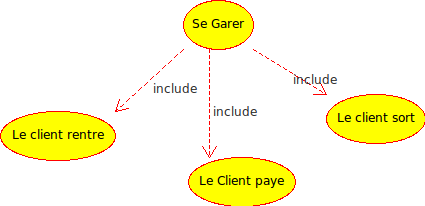
\includegraphics[scale=.7]{se_garer.png}
\end{figure}

\subsection{Collaboration}
\begin{figure}[!ht]
\centering
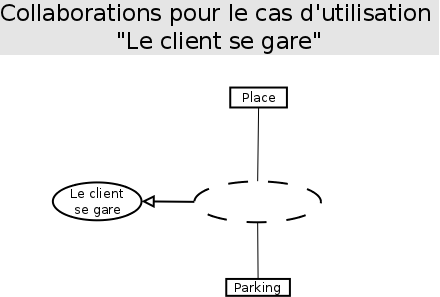
\includegraphics[scale=.5]{collaborations/_gare.png}
\end{figure}

\newpage

\section{Le client rentre}
\subsection{Cockburn}
\begin{description}
	\item[Cas d'utilisation] le client rentre
	\item[Acteur primaire] client
	\item[Acteur support] surveillant
	\item[Pr\'econdition] place libre dans le parking
	\item[Sc\'enario Primaire] \
	\begin{enumerate}
		\item Le client passe sous le syst\`eme de d\'etection de hauteur;
		\item le client passe sur la boucle au sol;
		\item le client appuye sur un bouton pour r\'ecup\'erer un ticket d'entr\'ee depuis
			le distributeur de ticket;
		\item la barri\`ere d'entrée se l\`eve;
		\item le client avance;
		\item la barri\`ere d'entrée d\'etecte le passage du client via la boucle au sol;
		\item la barri\`ere d'entrée se referme derri\`ere le client;
		\item le client se gare.
	\end{enumerate}
	\item[Postcondition] le client est rentr\'e dans le parking et a trouv\'e une place
	\item[Variantes] \
	\begin{enumerate}
		\item[1a] Le v\'ehicule est trop haut et ne peut rentrer dans
			le parking;
		\item[2a] le v\'ehicule est trop lourd: la borne d'entr\'ee le signale au client gr\^ace
                        \`a son \'ecran d'affichage. Le client peut alors pr\'evenir le 
                        surveillant via un interphone situ\'e sur la borne d'entr\'ee;
		\item[3a] \textbf{le client choisit de rentrer avec une carte};
		\item[3b] il n'y a plus de consommables, la barri\`ere d'entr\'ee pr\'evient
			le surveillant et demande au client de patienter via l'\'ecran d'affichage;
		\item[6a] la boucle au sol n'a pas d\'et\'ect\'e le passage d'un v\'ehicule
			en $5$ minutes, elle pr\'evient donc le surveillant puis se referme.
	\end{enumerate}
\end{description}

\newpage
\subsection{Diagramme d'activit\'es}
\begin{figure}[!ht]
\centering
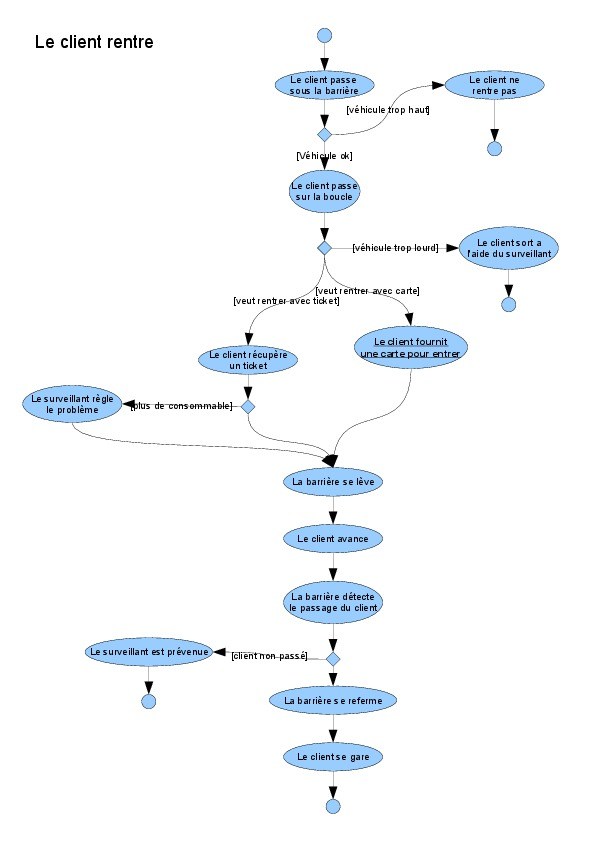
\includegraphics[scale=.7]{imgs/act_rentre.jpg}
\end{figure}
\newpage

\subsection{Collaboration}
\begin{figure}[!ht]
\centering
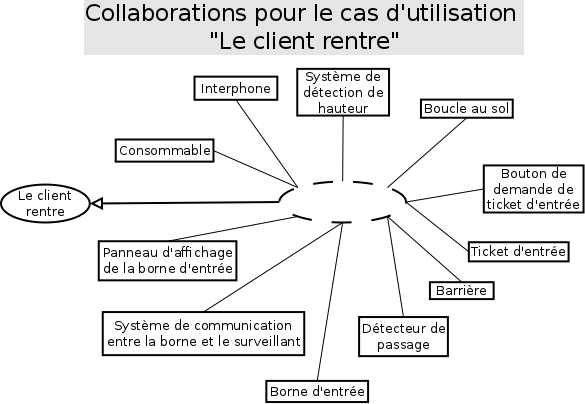
\includegraphics[scale=.5]{collaborations/_rentre.png}
\end{figure}

\newpage

\section{Le client choisit de rentrer avec une carte}
\subsection{Cockburn}
\begin{description}
	\item[Cas d'utilisation] le client choisit de rentrer avec une carte
	\item[Acteur primaire] client
	\item[Acteur support] surveillant
	\item[Pr\'econdition] place libre dans le parking
	\item[Sc\'enario Primaire] \
	\begin{enumerate}
		\item le client introduit une carte dans le lecteur de carte de la borne;
		\item la borne r\'ecup\`ere l'empreinte de la carte;
		\item la borne rend la carte
	\end{enumerate}
	\item[Postcondition] le client a r\'ecup\'er\'e sa carte et est pr\^et \`a rentrer.
	\item[Variantes] \
	\begin{enumerate}
		\item[1a] la carte n'est pas valide: soit ce n'est ni une carte bancaire
			ni une carte d'abonnement, soit c'est une carte r\'epertori\'ee
			comme \'etant perdue. Dans tous les cas, la borne pr\'evient le
			surveillant.
	\end{enumerate}
\end{description}

\subsection{Diagramme d'activit\'e}
\begin{figure}[!ht]
\centering
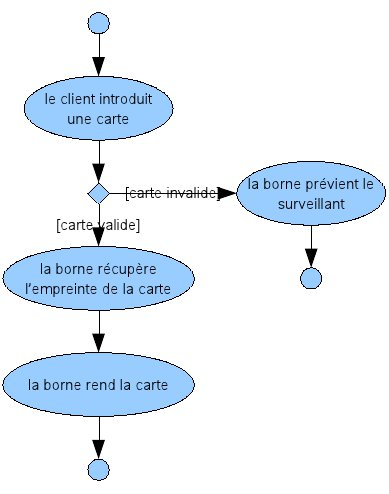
\includegraphics[scale=.7]{imgs/act_carterentrer.jpg}
\end{figure}

\subsection{Collaboration}
\begin{figure}[!ht]
\centering
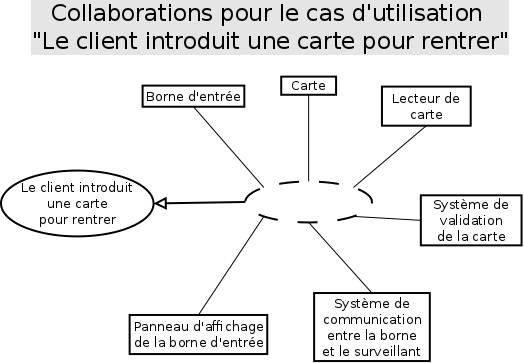
\includegraphics[scale=.5]{collaborations/_carte_entree.png}
\end{figure}

\newpage

\section{Le client sort}
\subsection{Cockburn}
\begin{description}
	\item[Cas d'utilisation] le client sort
	\item[Acteur primaire] client
	\item[Acteur support]
	\item[Pr\'econdition] le client est entr\'e dans le parking et poss\`ede un ticket de sortie
	\item[Sc\'enario Primaire] \
	\begin{enumerate}
		\item le client s'avance vers la premi\`ere barri\`ere;
		\item le client introduit son ticket de sortie dans le lecteur de ticket;
		\item la premi\`ere barri\`ere se l\`eve;
		\item le client s'avance sur la boucle;
		\item la premi\`ere barri\`ere de sortie se referme;
		\item la seconde barri\`ere de sortie se l\`eve;
		\item le client sort;
		\item la boucle d\'et\'ecte le passage du client;
		\item la deuxi\`eme barri\`ere s'abaisse.
	\end{enumerate}
	\item[Postcondition] le client est sorti.
	\item[Variantes] \
	\begin{enumerate}
		\item[2a] \textbf{Le client choisit de sortir avec une carte};
		\item[7a] la barri\`ere n'a pas d\'et\'ect\'e de v\'ehicule en $5$ minutes,
			elle pr\'evient donc le surveillant puis se referme.
	\end{enumerate}
\end{description}

\newpage
\subsection{Diagramme d'activit\'e}
\begin{figure}[!ht]
\centering
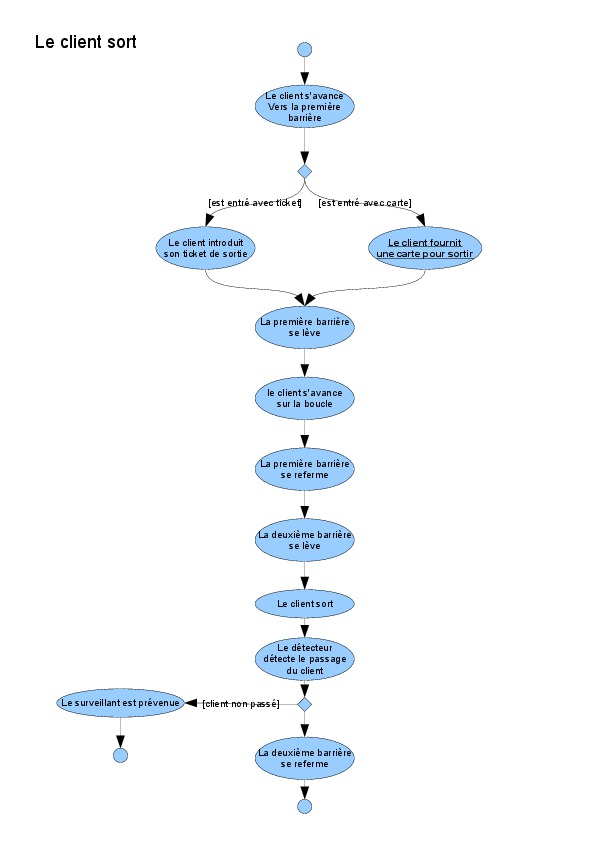
\includegraphics[scale=.7]{imgs/act_sort.jpg}
\end{figure}
\newpage

\subsection{Collaboration}
\begin{figure}[!ht]
\centering
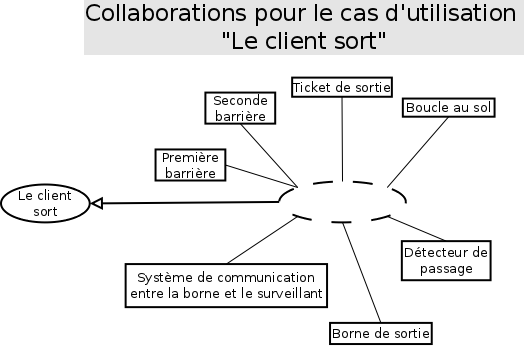
\includegraphics[scale=.5]{collaborations/_sort.png}
\end{figure}

\newpage

\section{Le client choisit de sortir avec une carte}
\subsection{Cockburn}
\begin{description}
	\item[Cas d'utilisation] le client choisit de sortir avec une carte
	\item[Acteur primaire] client
	\item[Acteur support] surveillant
	\item[Pr\'econdition] le client est entr\'e avec une carte et est \`a
		c\^ot\'e de la premi\`ere barri\`ere de sortie
	\item[Sc\'enario Primaire] \
	\begin{enumerate}
		\item Le client introduit une carte dans le lecteur;
		\item le lecteur envoie les informations relatives \`a la transaction
			\`a l'ordinateur du surveillant;
		\item le lecteur redonne la carte au client.
	\end{enumerate}
	\item[Postcondition] la transaction est enregistr\'ee
	\item[Variantes] \
	\begin{enumerate}
		\item[1a] la carte est invalide, la borne pr\'evient le surveillant;
	\end{enumerate}
\end{description}

\subsection{Diagramme d'activit\'e}
\begin{figure}[!ht]
\centering
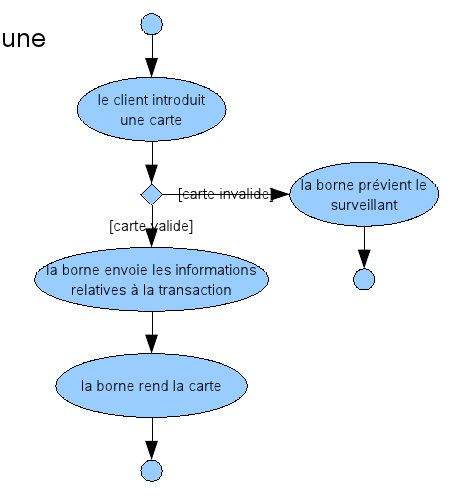
\includegraphics[scale=.7]{imgs/act_cartesortir.jpg}
\end{figure}

\subsection{Collaboration}
\begin{figure}[!ht]
\centering
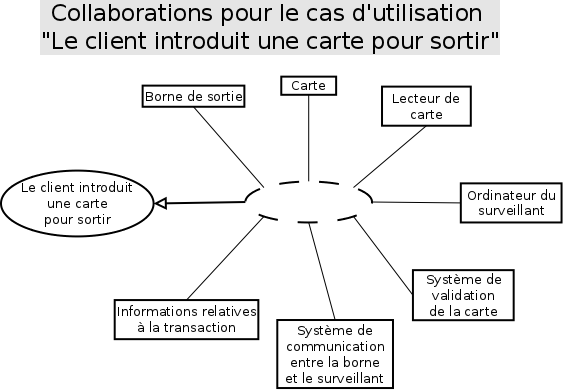
\includegraphics[scale=.5]{collaborations/_carte_sortie.png}
\end{figure}

\newpage


\section{Le client paye}
\subsection{Cockburn}
\begin{description}
	\item[Cas d'utilisation] le client paye
	\item[Acteur primaire] le client
	\item[Acteur support] le surveillant
	\item[Pr\'econdition] le client est entr\'e avec un ticket et est devant une caisse
	\item[Sc\'enario Primaire] \
	\begin{enumerate}
		\item le client fournit son ticket d'entr\'ee dans le lecteur de ticket;
		\item la caisse indique le montant \`a payer;
		\item \textbf{le client paye en liquide};
		\item le client r\'ecup\`ere un ticket de sortie dans le distributeur de ticket.
	\end{enumerate}
	\item[Postcondition] Le client a pay\'e et a un ticket de sortie
	\item[Variantes] \
	\begin{enumerate}
		\item[1a] le client a perdu son ticket d'entr\'ee, il appuye sur le
			bouton associ\'e et doit payer le prix maximum;
		\item[1b] le client donne son ticket au surveillant;
		\item[2a] le montant ne correspond pas ou ne s'affiche pas, le client
			pr\'evient le surveillant;
		\item[2b] le surveillant indique le montant \`a payer;
		\item[3a] \textbf{le client choisit de payer en carte};
		\item[3b] le client paye en ch\`eque au surveillant;
		\item[4a] il n'y a plus de consommable, le surveillant est pr\'evenu.
	\end{enumerate}
\end{description}

\subsection{Diagramme d'activit\'e}
\begin{figure}[!ht]
\centering
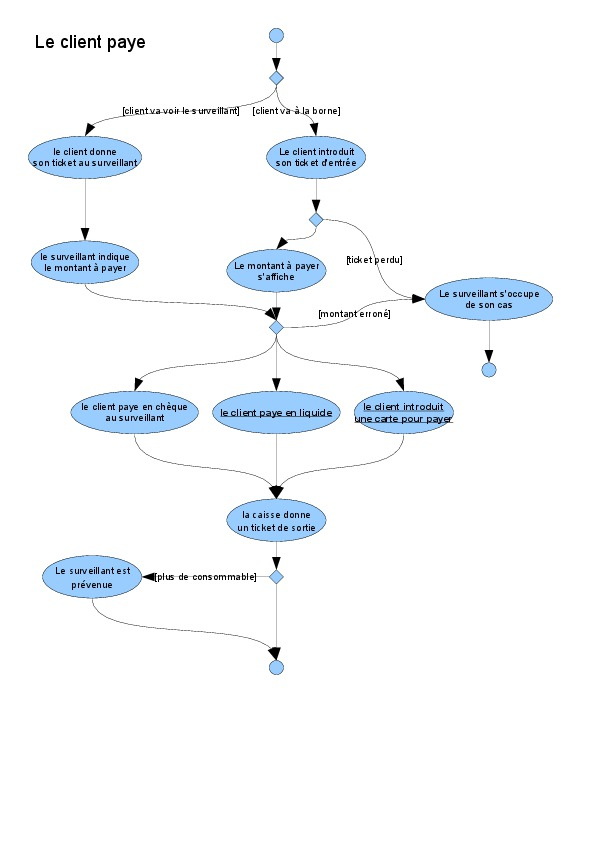
\includegraphics[scale=.7]{imgs/act_paye.jpg}
\end{figure}

\subsection{Collaboration}
\begin{figure}[!ht]
\centering
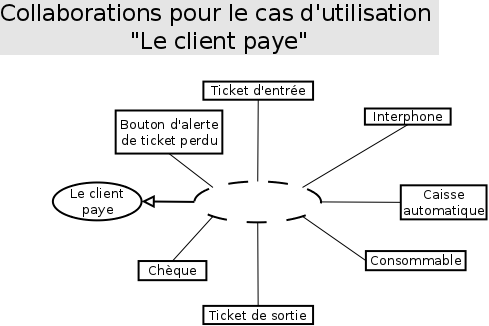
\includegraphics[scale=.5]{collaborations/_paye.png}
\end{figure}

\newpage

\section{le client paye en liquide}
\subsection{Cockburn}
\begin{description}
	\item[Cas d'utilisation] le client paye en liquide
	\item[Acteur primaire] le client
	\item[Acteur support] le surveillant
	\item[Pr\'econdition]
	\item[Sc\'enario Primaire] \
	\begin{enumerate}
		\item le client fournit de la monnaie \`a la caisse;
		\item la caisse rend la monnaie;
	\end{enumerate}
	\item[Postcondition] le client a pay\'e en liquide
	\item[Variantes] \
	\begin{enumerate}
		\item[1a] le client n'a pas fourni assez de monnaie et n'a
			pas interagi avec la machine pendant $5$ minutes: la
			caisse appelle le surveillant;
		\item[1b] la machines identifie des pi\`eces comme \'etant
			invalides: elle les rejette;
		\item[1c] le client appuye sur boutton pour annuler le
			payement et la machine lui rend les \'eventuelles
			pi\`eces qu'il aurait rendu;
		\item[2a] la caisse a un solde suffisant mais pas assez de
			monnaie: elle rend plus de monnaie, tout en indiquant au
			surveillant un manque d'esp\`eces;
		\item[2b] la caisse a un solde inf\'erieur \`a ce qu'elle doit
			rendre au client: elle pr\'evient le surveillant
	\end{enumerate}
\end{description}

\subsection{Diagramme d'activit\'e}
\begin{figure}[!ht]
\centering
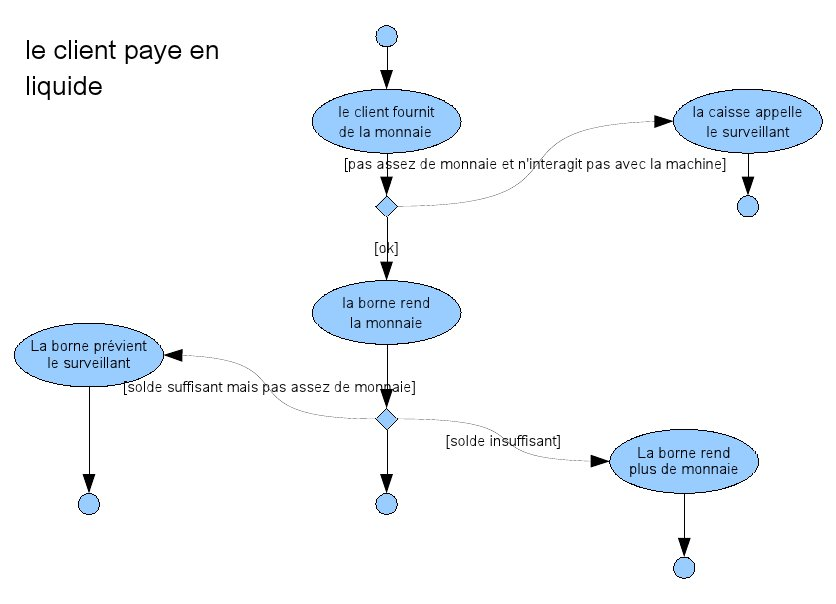
\includegraphics[scale=.5]{imgs/act_payerliquide.jpg}
\end{figure}

\subsection{Collaboration}
\begin{figure}[!ht]
\centering
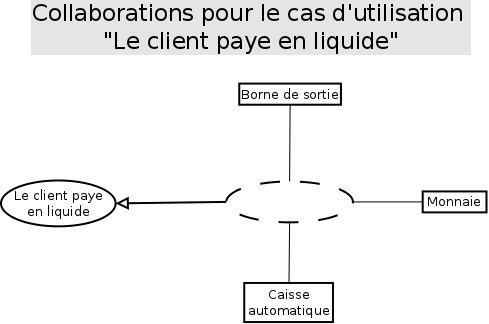
\includegraphics[scale=.5]{collaborations/_liquide.png}
\end{figure}

\newpage

\section{le client choisit de payer en carte}
\subsection{Cockburn}
\begin{description}
	\item[Cas d'utilisation] le client choisit de payer en carte
	\item[Acteur primaire] le client
	\item[Acteur support] le surveillant
	\item[Pr\'econdition] le client poss\`ede une carte
	\item[Sc\'enario Primaire] \
	\begin{enumerate}
		\item le client introduit une carte dans le lecteur de la borne;
		\item la borne calcule puis stocke la transaction \`a effectuer;
		\item la borne rend la carte
	\end{enumerate}
	\item[Postcondition] le client a pay\'e avec sa carte
	\item[Variantes] \
	\begin{enumerate}
		\item[1a] la carte est invalide; la borne pr\'evient le surveillant.
	\end{enumerate}
\end{description}
\subsection{Diagramme d'activit\'e}
\begin{figure}[!ht]
\centering
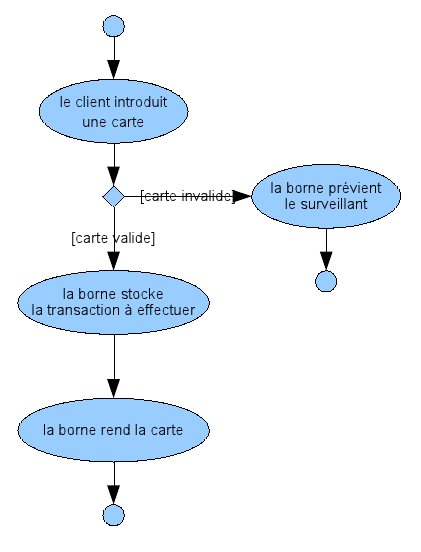
\includegraphics[scale=.7]{imgs/act_cartepayer.jpg}
\end{figure}

\subsection{Collaboration}
\begin{figure}[!ht]
\centering
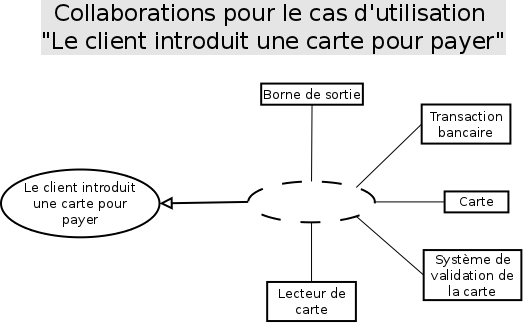
\includegraphics[scale=.5]{collaborations/_carte.png}
\end{figure}

\end{document}
